\section{Classification of Bd and Bs mesons}

The distinction between $B_d$ and $B_s$ mesons based on the associated event is a non-trivial problem.
Since both mesons have different masses, it is expected that there is some difference in the kinematics of the associated event.
Therefore, it is tested if a multivariate machine learning algorithm can spot these differences.
The algorithm of choice for this thesis is a DeepSet that is trained on simulated LHCb data.
As explained in \autoref{sec:DeepSet}, a DeepSet can handle data of variable length where the order of its elements should not change the result of the classification.
Therefore, DeepSets are ideal to classify $pp$-collision events that contain different amounts of particle tracks.
The DeepSets, trained here, ouput an estimated probability $\text{Prob}_{B_s}$ for each event that the signal $B$ is a $B_s$ meson.
Therefore, $1-\text{Prob}_{B_s}$ is the estimated probability that the signal $B$ is a $B_d$ meson.

The procedure of selecting important features is similar to the procedure described in \autoref{sec:SS_classifier}.
However, a DeepSet was trained on all features and the feature importances used here are the permutation importance of the ROC AUC and the permutation importance of the accuracy.
Again, features with the lowest feature importance scores are discarded until a reasonable amount of features is achieved.
The remaining 23 features are listed in \autoref{tab:B_features} and the corresponding feature importances are shown in \autoref{fig:B_importances}.

\begin{figure}
    \centering
    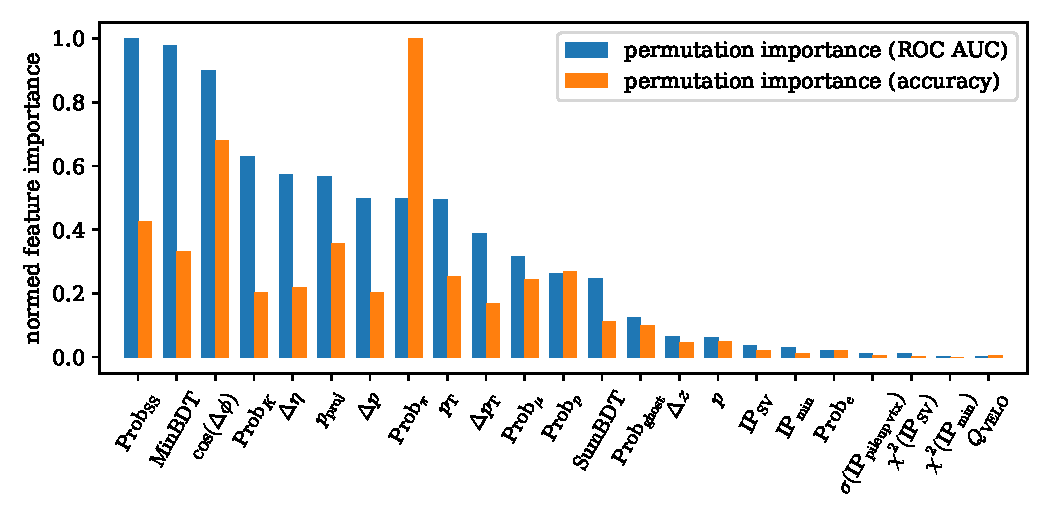
\includegraphics[width=\textwidth]{images/B_feature_importances.pdf}
    \caption{Calculated feature importances on the trained DeepSet. Shown are the permutation importances of the ROC AUC and the accuracy.}
    \label{fig:B_importances}
\end{figure}

\begin{table}
    \centering
    \caption{List of all features used to train the DeepSet for B meson classification.}
    \label{tab:B_features}
    \begin{tabular}{c c}
        \toprule
        feature & feature \\
        \midrule
        $p$                 & $\text{Prob}_\text{SS}$ \\ %"Tr_T_P","Tr_ProbSS"
        $p_\text{T}$        & $\text{PROBNN}_e$ \\ %"Tr_T_PT", "Tr_T_PROBNNe"
        $p_\text{proj}$     & $\text{PROBNN}_\text{ghost}$ \\ %"Tr_p_proj","Tr_T_PROBNNghost"
        $\Delta p_\text{T}$ & $\text{PROBNN}_k$ \\ %"Tr_diff_pt", "Tr_T_PROBNNk"
        $\Delta p$          & $\text{PROBNN}_\mu$ \\ %"Tr_diff_p","Tr_T_PROBNNmu"
        $\Delta z$          & $\text{PROBNN}_p$ \\ %"Tr_diff_z", "Tr_T_PROBNNp"
        $\cos(\Delta \phi)$ & $\text{PROBNN}_\pi$ \\ %"Tr_cos_diff_phi", "Tr_T_PROBNNpi"
        $\Delta \eta$       & IP\_trPUS \\ %"Tr_diff_eta", "Tr_T_IP_trPUS"
        IP\_trMother        & VeloCharge \\ %"Tr_T_IP_trMother",  "Tr_T_VeloCharge"
        IPCHI2\_trMother    & SumBDT\_ult \\ %"Tr_T_IPCHI2_trMother", "Tr_T_SumBDT_ult"
        MinIP               & MinBDT\_ult \\ %"Tr_T_MinIP", "Tr_T_MinBDT_ult"
        MinIPChi2           & \\ %"Tr_T_MinIPChi2"
        \bottomrule
    \end{tabular}
\end{table}

(Explain all features)....

The final DeepSet trained here consists of a $\phi$-network that extracts 64 features about each track and a $\rho$-network with a single output.
The $\phi$-network has an input layer of size 23 followed by 3 layers with of sizes 64, 128 and 64.
The $\rho$-network has an input layer of size 64 followed by 3 layers of sizes 128, 64 and 1.
All hidden layers use the activation function ReLU and have a dropout rate of $50\%$.
The output layer of the $\rho$-network uses the activation function Sigmoid.

This DeepSet is trained using the loss function binary cross entropy and the optimizer Adam.
From the $0.4$ million events in the dataset, $60\%$ are used for training and $40\%$ are used for validation of the trained model.
Using early stopping the training is stopped at iteration 600 after 50 iterations without improvement on the validation dataset.
The loss and the error rate for each iteration of the training of the DeepSet are shown in \autoref{fig:B_history}.

\begin{figure}
    \centering
    \begin{subfigure}{0.5\textwidth}
        \centering
        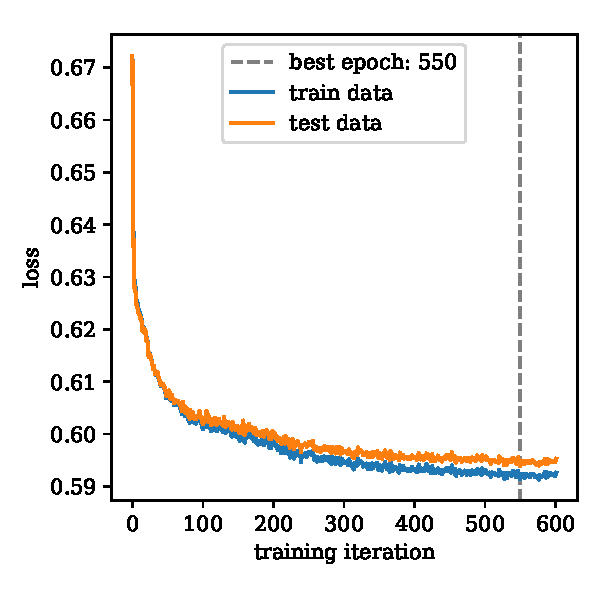
\includegraphics[width=\textwidth]{images/B_history_loss.pdf}
        \caption{binary cross entropy loss}
    \end{subfigure}%
    \begin{subfigure}{0.5\textwidth}
        \centering
        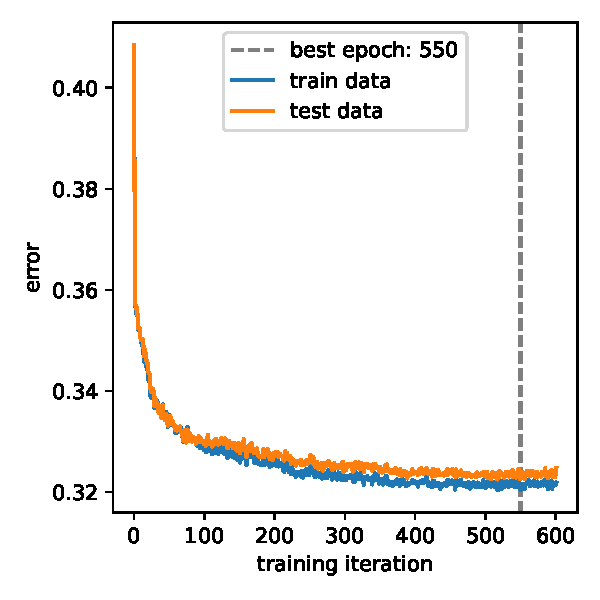
\includegraphics[width=\textwidth]{images/B_history_error.pdf}
        \caption{error rate}
    \end{subfigure}%
    \caption{Training performance of the DeepSet for $B$ meson classification.}
    \label{fig:B_history}
\end{figure}

To show the achieved separation of the $B$ mesons, histograms of $\text{Prob}_{B_s}$ split by the simulation ground truth are shown in \autoref{fig:B_output}.
The achieved ROC curve is shown in \autoref{fig:B_ROC} with a ROC AUC of $0.739$ on the test data and $0.742$ on the training data.
To estimate the generalization and overtraining of the model, each performance measure is calculated on both the test data and training data.

\begin{figure}
    \centering
    \begin{subfigure}{0.5\textwidth}
        \centering
        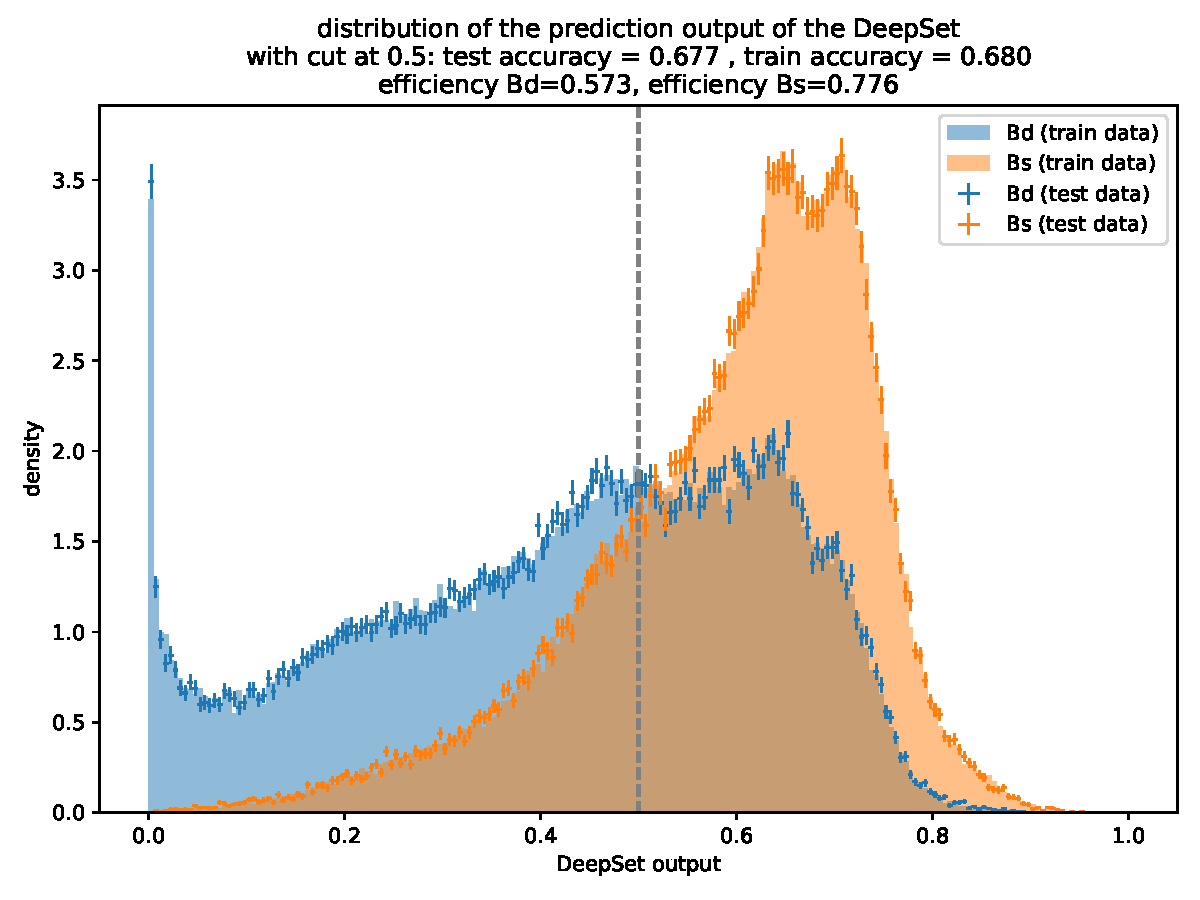
\includegraphics[width=\textwidth]{images/B_output.pdf}
        \caption{distribution of $\text{Prob}_{B_s}$}
        \label{fig:B_output}
    \end{subfigure}%
    \begin{subfigure}{0.5\textwidth}
        \centering
        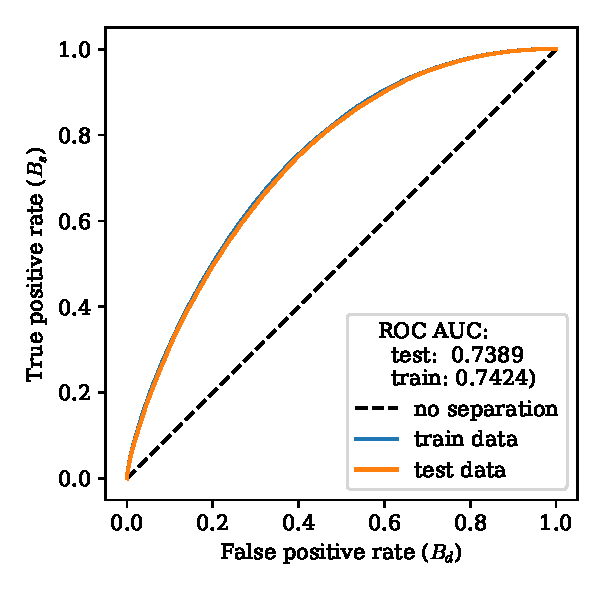
\includegraphics[width=\textwidth]{images/B_ROC.pdf}
        \caption{ROC curve}
        \label{fig:B_ROC}
    \end{subfigure}%
    \caption{\autoref{fig:B_output} shows the distribution of the DeepSet output split by the simulation ground truth. \autoref{fig:B_ROC} shows the ROC curve of the DeepSet output. Both figures show the DeepSet prediction for the test data and the training data.}
\end{figure}
